\documentclass{report}

\usepackage{geometry}
\geometry{a4paper,total={170mm,257mm},left=20mm,top=20mm}
\usepackage[utf8]{inputenc}
\usepackage{amsmath}
\usepackage{amsfonts}
\usepackage{amsthm}
\usepackage{amssymb}
\usepackage{bm}
\usepackage{graphicx}
\usepackage{paralist}
\usepackage[dvipsnames]{xcolor}
\usepackage{caption}
\usepackage{subcaption}
\usepackage{hyperref}
\hypersetup{urlbordercolor=ForestGreen,linkbordercolor=RoyalPurple}
\usepackage{tikz}
\usetikzlibrary{positioning}
\usetikzlibrary{intersections}
\usepackage{algpseudocode}
\usepackage{algorithm}
\usepackage{titling}
\usepackage{pgfplots}
\usepackage{fontawesome5}

%%% Tento soubor obsahuje definice různých užitečných maker a prostředí %%%
%%% Další makra připisujte sem, ať nepřekáží v ostatních souborech.     %%%

%%% Drobné úpravy stylu

% Tato makra přesvědčují mírně ošklivým trikem LaTeX, aby hlavičky kapitol
% sázel příčetněji a nevynechával nad nimi spoustu místa. Směle ignorujte.
\makeatletter
\def\@makechapterhead#1{
  {\parindent \z@ \raggedright \normalfont
   \Huge\bfseries \thechapter. #1
   \par\nobreak
   \vskip 20\p@
}}
\def\@makeschapterhead#1{
  {\parindent \z@ \raggedright \normalfont
   \Huge\bfseries #1
   \par\nobreak
   \vskip 20\p@
}}
\makeatother

% Toto makro definuje kapitolu, která není očíslovaná, ale je uvedena v obsahu.
\def\chapwithtoc#1{
\chapter*{#1}
\addcontentsline{toc}{chapter}{#1}
}

% Trochu volnější nastavení dělení slov, než je default.
\lefthyphenmin=2
\righthyphenmin=2

% Zapne černé "slimáky" na koncích řádků, které přetekly, abychom si
% jich lépe všimli.
\overfullrule=1mm

%%% Makra pro definice, věty, tvrzení, příklady, ... (vyžaduje baliček amsthm)

\theoremstyle{plain}
\newtheorem{veta}{Věta}
\newtheorem{lemma}[veta]{Lemma}
\newtheorem{tvrz}[veta]{Tvrzení}

\theoremstyle{plain}
\newtheorem{definice}{Definice}
\newtheorem*{pozor}{Pozorování}
\newtheorem*{cvic}{Cvičení}
\newtheorem*{fakt}{Fakt}

\theoremstyle{remark}
\newtheorem*{dusl}{Důsledek}
\newtheorem*{pozn}{Poznámka}
\newtheorem*{prikl}{Příklad}

\theoremstyle{plain}
\newtheorem{thm}{Theorem}
%\newtheorem{lemma}[thm]{Lemma}
\newtheorem{claim}[thm]{Claim}

\theoremstyle{plain}
\newtheorem{defn}{Definition}
\newtheorem*{observ}{Observation}
\newtheorem*{exerc}{Exercise}
\newtheorem*{fact}{Fact}

\theoremstyle{remark}
\newtheorem*{cor}{Corollary}
\newtheorem*{rem}{Remark}
\newtheorem*{example}{Example}


%%% Prostředí pro důkazy

\newenvironment{dukaz}{
  \par\medskip\noindent
  \textit{Důkaz}.
}{
\newline
\rightline{$\qedsymbol$}
}

\newenvironment{myproof}{
	\par\medskip\noindent
	\textit{Proof}.
}{
	\newline
	\rightline{$\qedsymbol$}
}


%%% Prostředí pro sazbu kódu, případně vstupu/výstupu počítačových
%%% programů. (Vyžaduje balíček fancyvrb -- fancy verbatim.)

\DefineVerbatimEnvironment{code}{Verbatim}{fontsize=\small, frame=single}

%%% Prostor reálných, resp. přirozených čísel
\newcommand{\R}{\mathbb{R}}
\newcommand{\N}{\mathbb{N}}
\newcommand{\Z}{\mathbb{Z}}

%%% Užitečné operátory pro statistiku a pravděpodobnost
\DeclareMathOperator{\pr}{\textsf{P}}
\DeclareMathOperator{\E}{\textsf{E}\,}
\DeclareMathOperator{\var}{\textrm{var}}
\DeclareMathOperator{\sd}{\textrm{sd}}

%%% Příkaz pro transpozici vektoru/matice
\newcommand{\T}[1]{#1^\top}

%%% Vychytávky pro matematiku
\newcommand{\goto}{\rightarrow}
\newcommand{\gotop}{\stackrel{P}{\longrightarrow}}
\newcommand{\maon}[1]{o(n^{#1})}
\newcommand{\abs}[1]{\left|{#1}\right|}
\newcommand{\dint}{\int_0^\tau\!\!\int_0^\tau}
\newcommand{\isqr}[1]{\frac{1}{\sqrt{#1}}}

%%% Vychytávky pro tabulky
\newcommand{\pulrad}[1]{\raisebox{1.5ex}[0pt]{#1}}
\newcommand{\mc}[1]{\multicolumn{1}{c}{#1}}


% set up \maketitle to accept a new item
\predate{\begin{center}\placetitlepicture\large}
	\postdate{\par\end{center}}

% commands for including the picture
\newcommand{\titlepicture}[2][]{%
	\renewcommand\placetitlepicture{%
		\includegraphics[#1]{#2}\par\medskip
	}%
}
\newcommand{\placetitlepicture}{} % initialization



\usepackage{babel}

\title{Polyhedral combinatorics}
\author{Tomáš Turek\thanks{Here are some of my notes taken from polyhedral combinatorics which was a part of course Mathematical programming and polyhedral combinatorics.\INFO}}
\titlepicture[width=4in]{res/polytope.pdf}
\date{\today}

\newcommand{\hpoly}[1]{$\mathcal{H}$-poly#1}
\newcommand{\vpoly}[1]{$\mathcal{V}$-poly#1}
\newcommand{\conv}{\mathtt{conv}}
\newcommand{\cone}{\mathtt{cone}}
\newcommand{\aff}{\mathtt{aff}}
\newcommand{\lin}{\mathtt{lin}}
\newcommand{\msum}{+_{\mathsf{M}}}
\newcommand{\pyr}{\mathtt{pyr}}
\newcommand{\bipyr}{\mathtt{bipyr}}

\begin{document}
	\maketitle
	\chapter{Definitions}

Reader may already know some basic definitions of polyhedrons and polytopes and also might be familiar with some basic theorems and characterization. But in the other case we will introduce some of these basics one more time. Also note that the main part is that we are considering somewhat basic linear program.

$$
\begin{aligned}
	\max c^{T} x \\
	A x \leq b
\end{aligned}
$$

\noindent Where we are considering a finite number of linear inequalities.

\section{Polyhedra and Polytopes}

The polyhedron created by such linear program is usually called \hpoly{hedron}. But we will formulate it more precisely.

\begin{defn}
	\hpoly{hedron} is prescribed as $\{x | A x \leq b\}$ where $A \in \R^{m \times n}$ and $b \in \R^{n}$.
\end{defn}

\begin{defn}[Minkowski sum]
	Minkowski sum of two sets $A,B$ denoted by $A \msum B$ is $\{a + b | a \in A, b \in B\}$.
\end{defn}

\begin{defn}[Combinations]
	Let $V$ be a finite set, then by the following statements

	\begin{enumerate}
			\item $x = \sum_{v_{i} \in V} \lambda_{i} v_{i}, \lambda_{i} \in \R${}
			\item $1 = \sum_{v_{i} \in V} \lambda_{i}$
			\item $0 \leq \lambda_{i}$
	\end{enumerate}

	\noindent we will define:

	\begin{itemize}
			\item Linear combination $\lin(V)$ as 1.
			\item Affine combination $\aff(V)$ as 1. and 2.
			\item Conic combination $\cone(V)$ as 1. and 3.
			\item Convex combination $\conv(V)$ as 1., 2. and 3.
	\end{itemize}
\end{defn}

\begin{figure}[!ht]\centering
	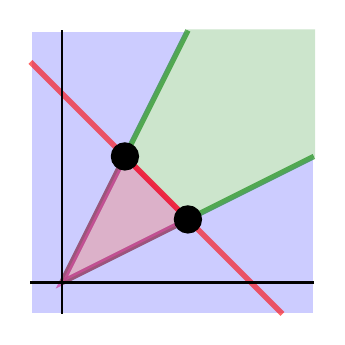
\begin{tikzpicture}[main/.style = {draw, circle, fill}, thick,
		comb/.style = {opacity = .6, line width = 2pt}, scale=.4]
			\draw[Blue!0, fill=Blue!20] (-1,-1) -- (-1,8) -- (8,8) -- (8,-1) -- cycle;
			\draw[Green!20, fill=Green!20] (0,0) -- (8,4) -- (8,8) -- (4,8) -- cycle;
			\draw[Green, comb] (4,8) -- (0,0);
			\draw[Green, comb] (8,4) -- (0,0);
			\draw[VioletRed, fill=VioletRed!50, comb] (0,0) -- (2,4) -- (4,2) -- cycle;
			\draw[Red, comb] (-1,7) -- (7,-1);
			\draw (-1,0) -- (8,0);
			\draw (0,-1) -- (0,8);
			\node[main] (1) at (4,2) {};
			\node[main] (2) at (2,4) {};
	\end{tikzpicture}
	\caption{Example of combinations, where $V$ are two points in $\R^{2}$, then we have their \textcolor{Blue}{linear combination}, \textcolor{Red}{affine combination}, \textcolor{Green}{conic combination} and \textcolor{VioletRed}{convex combination}.}
\end{figure}

\begin{defn}
	\vpoly{hedron} is defined as $\conv(V) \msum \cone(Y)$ where $V,Y$ are finite set of points.
\end{defn}

\begin{defn}
	Bounded-polyhedron is called \textbf{polytope}.
\end{defn}

This can be either visualized just by the definition or consider having a $n$-dimensional ball which is being cut by hyperplanes until no surface obtained by the ball itself persists.

\subsection{Examples of polytopes}

\subsubsection{Simplex}

This is a well known polytope which can be prescribed as follows. $k$-simplex is a convex combination of $k+1$ affine independent vertices.

\subsubsection{Cube}

Cube is even more known than the simplex. Already here we can see that it can be prescribed as \hpoly{tope} $\{x \in \R^{k} | 0 \leq x_{i} \leq 1\}$, but also as \vpoly{tope} $\conv(\{0,1\}^{k})$. This is quite essential, because we will see that \hpoly{hedra} and \vpoly{hedra} are equal.

\begin{figure}[!ht]\centering
	\begin{subfigure}{.45\textwidth}\centering
		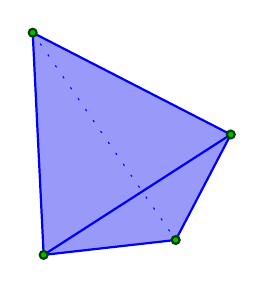
\begin{tikzpicture}
			[x={(0.454139cm, -0.658120cm)},
			y={(0.803660cm, 0.011660cm)},
			z={(-0.384562cm, -0.752823cm)},
			scale=2.000000,
			back/.style={loosely dotted, thin},
			edge/.style={color=blue!95!black, thick},
			facet/.style={fill=blue!95!black,fill opacity=0.400000},
			vertex/.style={inner sep=1pt,circle,draw=green!25!black,fill=green!75!black,thick}]
			\coordinate (-1.00000, 0.00000, 0.00000) at (-1.00000, 0.00000, 0.00000);
			\coordinate (0.00000, 0.00000, 1.00000) at (0.00000, 0.00000, 1.00000);
			\coordinate (0.00000, 1.00000, 0.00000) at (0.00000, 1.00000, 0.00000);
			\coordinate (1.00000, 0.00000, 0.00000) at (1.00000, 0.00000, 0.00000);
			\draw[edge,back] (-1.00000, 0.00000, 0.00000) -- (1.00000, 0.00000, 0.00000);
			\fill[facet] (0.00000, 1.00000, 0.00000) -- (-1.00000, 0.00000, 0.00000) -- (0.00000, 0.00000, 1.00000) -- cycle {};
			\fill[facet] (1.00000, 0.00000, 0.00000) -- (0.00000, 0.00000, 1.00000) -- (0.00000, 1.00000, 0.00000) -- cycle {};
			\draw[edge] (-1.00000, 0.00000, 0.00000) -- (0.00000, 0.00000, 1.00000);
			\draw[edge] (-1.00000, 0.00000, 0.00000) -- (0.00000, 1.00000, 0.00000);
			\draw[edge] (0.00000, 0.00000, 1.00000) -- (0.00000, 1.00000, 0.00000);
			\draw[edge] (0.00000, 0.00000, 1.00000) -- (1.00000, 0.00000, 0.00000);
			\draw[edge] (0.00000, 1.00000, 0.00000) -- (1.00000, 0.00000, 0.00000);
			\node[vertex] at (-1.00000, 0.00000, 0.00000)     {};
			\node[vertex] at (0.00000, 0.00000, 1.00000)     {};
			\node[vertex] at (0.00000, 1.00000, 0.00000)     {};
			\node[vertex] at (1.00000, 0.00000, 0.00000)     {};
		\end{tikzpicture}
		\caption{3 dimensional simplex}
	\end{subfigure}
	\begin{subfigure}{.45\textwidth}\centering{}
		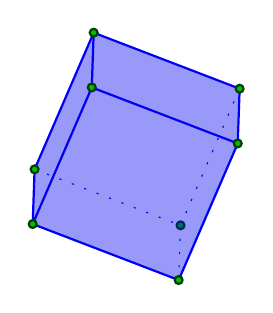
\begin{tikzpicture}
			[x={(0.926869cm, -0.355696cm)},
			y={(0.375194cm, 0.867588cm)},
			z={(-0.011997cm, -0.347523cm)},
			scale=2.000000,
			back/.style={loosely dotted, thin},
			edge/.style={color=blue!95!black, thick},
			facet/.style={fill=blue!95!black,fill opacity=0.400000},
			vertex/.style={inner sep=1pt,circle,draw=green!25!black,fill=green!75!black,thick}]
			\coordinate (0.00000, 0.00000, 0.00000) at (0.00000, 0.00000, 0.00000);
			\coordinate (0.00000, 0.00000, 1.00000) at (0.00000, 0.00000, 1.00000);
			\coordinate (0.00000, 1.00000, 0.00000) at (0.00000, 1.00000, 0.00000);
			\coordinate (0.00000, 1.00000, 1.00000) at (0.00000, 1.00000, 1.00000);
			\coordinate (1.00000, 0.00000, 0.00000) at (1.00000, 0.00000, 0.00000);
			\coordinate (1.00000, 0.00000, 1.00000) at (1.00000, 0.00000, 1.00000);
			\coordinate (1.00000, 1.00000, 0.00000) at (1.00000, 1.00000, 0.00000);
			\coordinate (1.00000, 1.00000, 1.00000) at (1.00000, 1.00000, 1.00000);
			\draw[edge,back] (0.00000, 0.00000, 0.00000) -- (1.00000, 0.00000, 0.00000);
			\draw[edge,back] (1.00000, 0.00000, 0.00000) -- (1.00000, 0.00000, 1.00000);
			\draw[edge,back] (1.00000, 0.00000, 0.00000) -- (1.00000, 1.00000, 0.00000);
			\node[vertex] at (1.00000, 0.00000, 0.00000)     {};
			\fill[facet] (1.00000, 1.00000, 1.00000) -- (0.00000, 1.00000, 1.00000) -- (0.00000, 0.00000, 1.00000) -- (1.00000, 0.00000, 1.00000) -- cycle {};
			\fill[facet] (1.00000, 1.00000, 1.00000) -- (0.00000, 1.00000, 1.00000) -- (0.00000, 1.00000, 0.00000) -- (1.00000, 1.00000, 0.00000) -- cycle {};
			\fill[facet] (0.00000, 1.00000, 1.00000) -- (0.00000, 0.00000, 1.00000) -- (0.00000, 0.00000, 0.00000) -- (0.00000, 1.00000, 0.00000) -- cycle {};
			\draw[edge] (0.00000, 0.00000, 0.00000) -- (0.00000, 0.00000, 1.00000);
			\draw[edge] (0.00000, 0.00000, 0.00000) -- (0.00000, 1.00000, 0.00000);
			\draw[edge] (0.00000, 0.00000, 1.00000) -- (0.00000, 1.00000, 1.00000);
			\draw[edge] (0.00000, 0.00000, 1.00000) -- (1.00000, 0.00000, 1.00000);
			\draw[edge] (0.00000, 1.00000, 0.00000) -- (0.00000, 1.00000, 1.00000);
			\draw[edge] (0.00000, 1.00000, 0.00000) -- (1.00000, 1.00000, 0.00000);
			\draw[edge] (0.00000, 1.00000, 1.00000) -- (1.00000, 1.00000, 1.00000);
			\draw[edge] (1.00000, 0.00000, 1.00000) -- (1.00000, 1.00000, 1.00000);
			\draw[edge] (1.00000, 1.00000, 0.00000) -- (1.00000, 1.00000, 1.00000);
			\node[vertex] at (0.00000, 0.00000, 0.00000)     {};
			\node[vertex] at (0.00000, 0.00000, 1.00000)     {};
			\node[vertex] at (0.00000, 1.00000, 0.00000)     {};
			\node[vertex] at (0.00000, 1.00000, 1.00000)     {};
			\node[vertex] at (1.00000, 0.00000, 1.00000)     {};
			\node[vertex] at (1.00000, 1.00000, 0.00000)     {};
			\node[vertex] at (1.00000, 1.00000, 1.00000)     {};
		\end{tikzpicture}
		\caption{3 dimensional cube}
	\end{subfigure}
\end{figure}

\subsubsection{Pyramids and other creations}

Also we will show us a simple way how to create new polytopes. That is imagine we have a polytope $P$ and put it in a higher dimension, then by adding one point above the $P$ and creating a convex hull of $P$ and the point we obtain a so called pyramid. We may also denote it as $\pyr(P)$. Similarly if we would take two points, where one is above and the second one is below the given $P$ we get bipyramid or $\bipyr(P)$.

Last creation we will show us right now is if we would take a parallel copy of the polytope $P$, that is to some other parallel hyperplane and connect these two together. This way we obtain a prism.

\begin{figure}[!ht]\centering
	\begin{subfigure}{.3\textwidth}\centering
			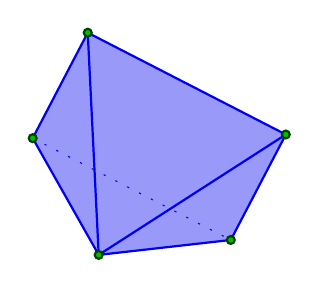
\begin{tikzpicture}
				[x={(0.454139cm, -0.658120cm)},
				y={(0.803660cm, 0.011660cm)},
				z={(-0.384562cm, -0.752823cm)},
				scale=2.000000,
				back/.style={loosely dotted, thin},
				edge/.style={color=blue!95!black, thick},
				facet/.style={fill=blue!95!black,fill opacity=0.400000},
				vertex/.style={inner sep=1pt,circle,draw=green!25!black,fill=green!75!black,thick}]
			\coordinate (-1.00000, 0.00000, 0.00000) at (-1.00000, 0.00000, 0.00000);
			\coordinate (0.00000, -1.00000, 0.00000) at (0.00000, -1.00000, 0.00000);
			\coordinate (0.00000, 0.00000, 1.00000) at (0.00000, 0.00000, 1.00000);
			\coordinate (0.00000, 1.00000, 0.00000) at (0.00000, 1.00000, 0.00000);
			\coordinate (1.00000, 0.00000, 0.00000) at (1.00000, 0.00000, 0.00000);
			\draw[edge,back] (0.00000, -1.00000, 0.00000) -- (1.00000, 0.00000, 0.00000);
			\fill[facet] (0.00000, 0.00000, 1.00000) -- (-1.00000, 0.00000, 0.00000) -- (0.00000, -1.00000, 0.00000) -- cycle {};
			\fill[facet] (0.00000, 1.00000, 0.00000) -- (-1.00000, 0.00000, 0.00000) -- (0.00000, 0.00000, 1.00000) -- cycle {};
			\fill[facet] (1.00000, 0.00000, 0.00000) -- (0.00000, 0.00000, 1.00000) -- (0.00000, 1.00000, 0.00000) -- cycle {};
			\draw[edge] (-1.00000, 0.00000, 0.00000) -- (0.00000, -1.00000, 0.00000);
			\draw[edge] (-1.00000, 0.00000, 0.00000) -- (0.00000, 0.00000, 1.00000);
			\draw[edge] (-1.00000, 0.00000, 0.00000) -- (0.00000, 1.00000, 0.00000);
			\draw[edge] (0.00000, -1.00000, 0.00000) -- (0.00000, 0.00000, 1.00000);
			\draw[edge] (0.00000, 0.00000, 1.00000) -- (0.00000, 1.00000, 0.00000);
			\draw[edge] (0.00000, 0.00000, 1.00000) -- (1.00000, 0.00000, 0.00000);
			\draw[edge] (0.00000, 1.00000, 0.00000) -- (1.00000, 0.00000, 0.00000);
			\node[vertex] at (-1.00000, 0.00000, 0.00000)     {};
			\node[vertex] at (0.00000, -1.00000, 0.00000)     {};
			\node[vertex] at (0.00000, 0.00000, 1.00000)     {};
			\node[vertex] at (0.00000, 1.00000, 0.00000)     {};
			\node[vertex] at (1.00000, 0.00000, 0.00000)     {};
		\end{tikzpicture}
		\caption{Pyramid}
	\end{subfigure}
	\begin{subfigure}{.3\textwidth}\centering
			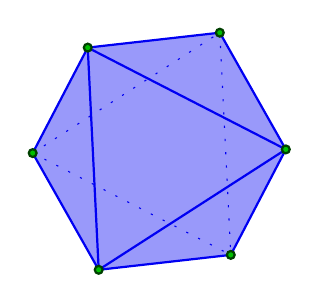
\begin{tikzpicture}
			[x={(0.454139cm, -0.658120cm)},
			y={(0.803660cm, 0.011660cm)},
			z={(-0.384562cm, -0.752823cm)},
			scale=2.000000,
			back/.style={loosely dotted, thin},
			edge/.style={color=blue!95!black, thick},
			facet/.style={fill=blue!95!black,fill opacity=0.400000},
			vertex/.style={inner sep=1pt,circle,draw=green!25!black,fill=green!75!black,thick}]
		\coordinate (-1.00000, 0.00000, 0.00000) at (-1.00000, 0.00000, 0.00000);
		\coordinate (0.00000, -1.00000, 0.00000) at (0.00000, -1.00000, 0.00000);
		\coordinate (0.00000, 0.00000, -1.00000) at (0.00000, 0.00000, -1.00000);
		\coordinate (0.00000, 0.00000, 1.00000) at (0.00000, 0.00000, 1.00000);
		\coordinate (0.00000, 1.00000, 0.00000) at (0.00000, 1.00000, 0.00000);
		\coordinate (1.00000, 0.00000, 0.00000) at (1.00000, 0.00000, 0.00000);
		\draw[edge,back] (0.00000, -1.00000, 0.00000) -- (0.00000, 0.00000, -1.00000);
		\draw[edge,back] (0.00000, -1.00000, 0.00000) -- (1.00000, 0.00000, 0.00000);
		\draw[edge,back] (0.00000, 0.00000, -1.00000) -- (1.00000, 0.00000, 0.00000);
		\fill[facet] (0.00000, 1.00000, 0.00000) -- (-1.00000, 0.00000, 0.00000) -- (0.00000, 0.00000, 1.00000) -- cycle {};
		\fill[facet] (0.00000, 0.00000, 1.00000) -- (-1.00000, 0.00000, 0.00000) -- (0.00000, -1.00000, 0.00000) -- cycle {};
		\fill[facet] (0.00000, 1.00000, 0.00000) -- (-1.00000, 0.00000, 0.00000) -- (0.00000, 0.00000, -1.00000) -- cycle {};
		\fill[facet] (1.00000, 0.00000, 0.00000) -- (0.00000, 0.00000, 1.00000) -- (0.00000, 1.00000, 0.00000) -- cycle {};
		\draw[edge] (-1.00000, 0.00000, 0.00000) -- (0.00000, -1.00000, 0.00000);
		\draw[edge] (-1.00000, 0.00000, 0.00000) -- (0.00000, 0.00000, -1.00000);
		\draw[edge] (-1.00000, 0.00000, 0.00000) -- (0.00000, 0.00000, 1.00000);
		\draw[edge] (-1.00000, 0.00000, 0.00000) -- (0.00000, 1.00000, 0.00000);
		\draw[edge] (0.00000, -1.00000, 0.00000) -- (0.00000, 0.00000, 1.00000);
		\draw[edge] (0.00000, 0.00000, -1.00000) -- (0.00000, 1.00000, 0.00000);
		\draw[edge] (0.00000, 0.00000, 1.00000) -- (0.00000, 1.00000, 0.00000);
		\draw[edge] (0.00000, 0.00000, 1.00000) -- (1.00000, 0.00000, 0.00000);
		\draw[edge] (0.00000, 1.00000, 0.00000) -- (1.00000, 0.00000, 0.00000);
		\node[vertex] at (-1.00000, 0.00000, 0.00000)     {};
		\node[vertex] at (0.00000, -1.00000, 0.00000)     {};
		\node[vertex] at (0.00000, 0.00000, -1.00000)     {};
		\node[vertex] at (0.00000, 0.00000, 1.00000)     {};
		\node[vertex] at (0.00000, 1.00000, 0.00000)     {};
		\node[vertex] at (1.00000, 0.00000, 0.00000)     {};
		\end{tikzpicture}
		\caption{Bipyramid}
	\end{subfigure}
	\begin{subfigure}{.3\textwidth}\centering{}
		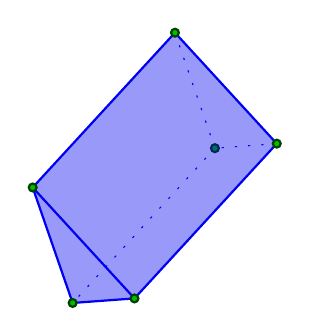
\begin{tikzpicture}
			[x={(0.181209cm, -0.523814cm)},
			y={(0.742124cm, -0.482509cm)},
			z={(-0.645302cm, -0.702000cm)},
			scale=1.400000,
			back/.style={loosely dotted, thin},
			edge/.style={color=blue!95!black, thick},
			facet/.style={fill=blue!95!black,fill opacity=0.400000},
			vertex/.style={inner sep=1pt,circle,draw=green!25!black,fill=green!75!black,thick}]
			\coordinate (-1.00000, 0.00000, 0.00000) at (-1.00000, 0.00000, 0.00000);
			\coordinate (-1.00000, 0.00000, 2.00000) at (-1.00000, 0.00000, 2.00000);
			\coordinate (0.00000, 1.00000, 0.00000) at (0.00000, 1.00000, 0.00000);
			\coordinate (0.00000, 1.00000, 2.00000) at (0.00000, 1.00000, 2.00000);
			\coordinate (1.00000, 0.00000, 0.00000) at (1.00000, 0.00000, 0.00000);
			\coordinate (1.00000, 0.00000, 2.00000) at (1.00000, 0.00000, 2.00000);
			\draw[edge,back] (-1.00000, 0.00000, 0.00000) -- (1.00000, 0.00000, 0.00000);
			\draw[edge,back] (0.00000, 1.00000, 0.00000) -- (1.00000, 0.00000, 0.00000);
			\draw[edge,back] (1.00000, 0.00000, 0.00000) -- (1.00000, 0.00000, 2.00000);
			\node[vertex] at (1.00000, 0.00000, 0.00000)     {};
			\fill[facet] (0.00000, 1.00000, 2.00000) -- (-1.00000, 0.00000, 2.00000) -- (-1.00000, 0.00000, 0.00000) -- (0.00000, 1.00000, 0.00000) -- cycle {};
			\fill[facet] (1.00000, 0.00000, 2.00000) -- (-1.00000, 0.00000, 2.00000) -- (0.00000, 1.00000, 2.00000) -- cycle {};
			\draw[edge] (-1.00000, 0.00000, 0.00000) -- (-1.00000, 0.00000, 2.00000);
			\draw[edge] (-1.00000, 0.00000, 0.00000) -- (0.00000, 1.00000, 0.00000);
			\draw[edge] (-1.00000, 0.00000, 2.00000) -- (0.00000, 1.00000, 2.00000);
			\draw[edge] (-1.00000, 0.00000, 2.00000) -- (1.00000, 0.00000, 2.00000);
			\draw[edge] (0.00000, 1.00000, 0.00000) -- (0.00000, 1.00000, 2.00000);
			\draw[edge] (0.00000, 1.00000, 2.00000) -- (1.00000, 0.00000, 2.00000);
			\node[vertex] at (-1.00000, 0.00000, 0.00000)     {};
			\node[vertex] at (-1.00000, 0.00000, 2.00000)     {};
			\node[vertex] at (0.00000, 1.00000, 0.00000)     {};
			\node[vertex] at (0.00000, 1.00000, 2.00000)     {};
			\node[vertex] at (1.00000, 0.00000, 2.00000)     {};
		\end{tikzpicture}
		\caption{Prism}
	\end{subfigure}
\end{figure}

\begin{thm}[Minkowski-Weyl]
	$P$ is \hpoly{hedron} $\iff$ it is a \vpoly{hedron}.
\end{thm}

\begin{proof}[Sketch of the proof]
	"$\Rightarrow$" We will gradually make the polyhedron more non-general and then consider a simple case. So WLOG:

	\begin{enumerate}
		\item $P$ is full-dimensional. Where dimension is defined as dimension of the smallest affine space containing it.
		\item $P$ is pointed, that is it does not contain a line. -- If it contains a line we can split it by an orthogonal hyperplane, inductively use Minkowski-Weyl theorem and then extend $Y$ by rays to both sides of the hyperplane. Use theorem \ref{pointed-P}.
		\item $V = \emptyset$ -- Use trick which is called \textbf{Homogenization} or \textbf{Homogenized cone} which is that $P : Ax \leq b$ create $P' : Ax - bz \leq 0$ and $z \geq 0$. So for $z = 1$ we have original $P$ and then for all others $z$ we have scaled copy of $P$. After this trick we use Minkowski-Weyl for this cone and create $V$ by the points for which $z > 0$ and $Y$ from poitns for which $z = 0$.
		\item $P$ is a polytope. And with that we use claim \ref{polytope}.
	\end{enumerate}

	"$\Leftarrow$" Set $P = \{x | x = \sum \lambda_{i} x_{i}, 1 = \sum \lambda_{i}, 0 \leq \lambda_{i}\}$ which is a \hpoly{tope}. By also using Fourier Monskin split to positive, 0 and negative koeficients.
\end{proof}

\begin{thm}
	$P$ is a pointed $\iff$ it has an extreme point.
	\label{pointed-P}
\end{thm}

\begin{proof}
	If there is a line and we have extreme point we can shift the line so it goes through the extreme point. But now the line representing the optimization function is either parallel hence it is not an extreme point or not parallel which also implies it is not an extreme point.
\end{proof}

\begin{claim}
Lets have polytope $P = \{x | A x \leq b\}$ and $V$ be the set of extreme point of $P$. Then $P = \conv(V)$.
	\label{polytope}
\end{claim}

\begin{proof}
	"$P \supseteq \conv(V)$" Is easy. So see "$P \subseteq \conv(V)$". Suppose it is not true. Take any such $x$ and find a hyperplane separating $\conv(V)$ and $x$ which can be done by Hyperplane separation lemma (that is choosing shortest segment and creating an orthogonal hyperplane between them). Then the optimum of the direction set by the norm of this hyperplane gives an extreme point, which is a contradiction.
\end{proof}

From the main theorem we may see that from mathematical perspective both \hpoly{hedrons} and \vpoly{hedrons} are the same. But for computer scientists it is pretty much the opposite. Consider solving an LP. Given linear inequalities it takes some time to solve it, but if we have all vertices we can just check every one of them if it is optimum. Also iff we would like to see an intersection of two polytopes $P,Q$ it is the opposite. That is we can just add all inequalities together and obtain their intersection. On the other hand for convex points it is known to be NP hard.

\begin{fact}
	For polytope $P \subseteq \R^{d}$ given by $n$ inequalitites it has $\leq n^{\lfloor d/2 \rfloor}$ vertices.
\end{fact}

\section{Faces of polytopes (polyhedrons)}

\begin{defn}
	Let $P$ be a polyhedron. An inequality $\alpha^{T} x \leq \beta$ is \textbf{valid} for $P$ if $P \cap \{x | \alpha^{T} x \leq \beta\} = P$.
\end{defn}

\begin{defn}
	Let $P$ be a polyhedron and $\alpha^{T} x \leq \beta$ a valid inequality. Then $F = P \cap \{x | \alpha^{T} x = \beta\}$ is called a \textbf{face} of $P$.
\end{defn}

Keep in mind that there are two special cases that are usualy called \textit{trivial} faces. Consider $\bm{0}^{T} x \leq 0$ and $\bm{0}^{T} x \leq 1$ which are valid and the first create a face $P$, whereas the second $\emptyset$. The other faces are called \textit{non-trivial}.

\begin{thm}
	Let $P$ be a polytope $A x \leq b$ then $F$ is a face of $P$ \ifft $F = \{x | A' x = b'\} \cap P$ for some subset of "original inequalities". Or sometimes called a subsystem.
\end{thm}

\begin{proof}
	"$\Rightarrow$" Let $F$ be a face of $P$. Then $\exists$ valid $c^{T} x \leq \delta$ such that $F = P \cap \{x | c^{T} x = \delta\}$. In the dual LP for $\max c^{T} x$ s.t. $A x \leq b$ let $y^{\ast}$ be optimum and let $I = \{i | y_{i} = 0\}$. Then $F \subseteq P \cap \{x | a_{i}^{T} x = b, i \in I\}$ can be seen from the fact about complementarity \ref{complementarity}. But also the other inclusion holds thus  $F = P \cap \{x | a_{i}^{T} x = b, i \in I\}$.
	
	"$\Leftarrow$" Let $F = P \cap \{x | a_{i}^{T} x = b\}$. Then claim $F$ is a face can be seen by setting $c := \sum_{i \in I} a_{i}$ and $\delta := \sum_{i \in I} b_{i}$. See that $c^{T} x \leq \delta$ is valid and it prescribe a face.
\end{proof}

\begin{fact}[Complementarity]
	For LP $\max c^{T}x$ s.t. $A x \leq b$ and its dual $\min b^{T} y$ s.t. $A^{T} y = c, y \geq 0$. Let $x^{\ast}$ and $y^{\ast}$ be primal (dual) optimum solutions, then if $y_{i}^{\ast} > 0$ then $a_{i}^{T} x^{\ast} = b_{i}$.
\end{fact}

\begin{proof}
	$c^{T}x = y^{T}Ax = y^{T}b$ therefore $y^{T}(Ax + b) = 0$ so component wise it must be 0 $\forall i$, hence either $y_{i} = 0$ or $(a_{i}x - b_{i}) =0$.
\end{proof}

Also faces of polyhedron are also polyhdra as well. Face of a face is also a face and intersection of faces is a face. These are some properties which can be observed. Lastly we may look at special faces by their dimensions which are prescribed in table \ref{faces}.

\begin{table}[!ht]\centering
	\begin{tabular}{c|c}
		dimension & face \\
		\hline
		0 & vertices \\
		1 & edges \\
		$\vdots$ & $\vdots$ \\
		$\dim(P) - 2$ & ridges \\
		$\dim(P) - 1$ & facets
	\end{tabular}
	\caption{Most important faces.}
	\label{faces}
\end{table}

\subsection{Face lettice}

Let $\mathcal{F}$ be the set of faces of $P$, then $(\mathcal{F}, \subseteq)$ is called the \textit{face lattice}. The fact that it is called lattice is due to the properties it has. Moreover it has some other properties, which are sometimes called as a graded lattice (elements can be dividided by their grades). Also for all pairs it has its sublattice.

\begin{example}
	See an easy example of 2-dimensional cube and its lattice on Fig. \ref{lattice}.

	\begin{figure}[!ht]\centering
		\begin{subfigure}{.3\textwidth}\centering
			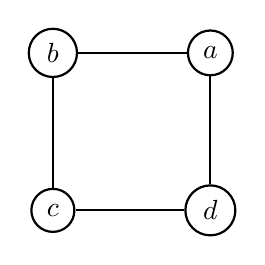
\begin{tikzpicture}[node distance = 20mm, main/.style = {draw, circle}, thick]
				\node[main] (a) {$a$};
				\node[main, left of = a] (b) {$b$};
				\node[main, below of = b] (c) {$c$};
				\node[main, below of = a] (d) {$d$};
				\draw (a) -- (b);
				\draw (b) -- (c);
				\draw (c) -- (d);
				\draw (d) -- (a);
			\end{tikzpicture}
			\caption{2-dimensional cube}
		\end{subfigure}
		\begin{subfigure}{.65\textwidth}\centering{}
			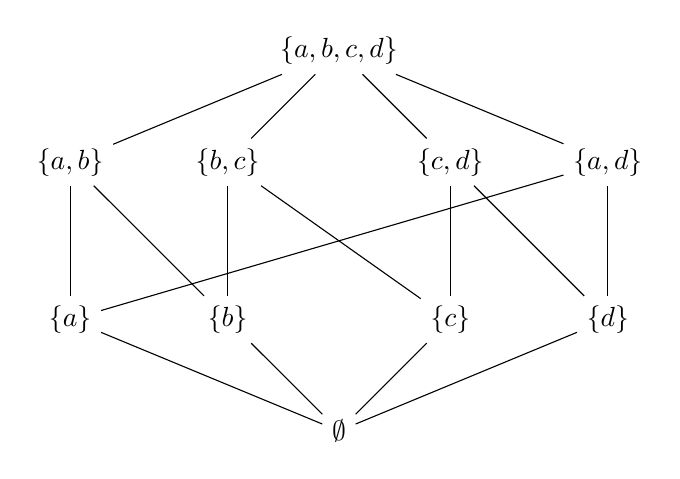
\begin{tikzpicture}[node distance = 20mm]
				\node (P) {$\{a,b,c,d\}$};
				\node[below left of = P] (bc) {$\{b,c\}$};
				\node[below right of = P] (cd) {$\{c,d\}$};
				\node[right of = cd] (da) {$\{a,d\}$};
				\node[left of = bc] (ab) {$\{a,b\}$};
				\node[below of = ab] (a) {$\{a\}$};
				\node[below of = bc] (b) {$\{b\}$};
				\node[below of = cd] (c) {$\{c\}$};
				\node[below of = da] (d) {$\{d\}$};
				\node[below left of = c] (empty) {$\emptyset$};
				\draw (P) -- (ab);
				\draw (P) -- (bc);
				\draw (P) -- (cd);
				\draw (P) -- (da);
				\draw (a) -- (ab);
				\draw (b) -- (ab);
				\draw (c) -- (bc);
				\draw (b) -- (bc);
				\draw (d) -- (cd);
				\draw (c) -- (cd);
				\draw (a) -- (da);
				\draw (d) -- (da);
				\draw (empty) -- (a);
				\draw (empty) -- (b);
				\draw (empty) -- (c);
				\draw (empty) -- (d);
			\end{tikzpicture}
			\caption{and its lattice.}
		\end{subfigure}
		\caption{Example of face lattice.}
		\label{lattice}
	\end{figure}
\end{example}

\subsection{Polar duality}

For a polytope $P$ which is described as $A x \leq \bm{1}$ and also by $\conv(V)$ we have the polar dual $P^{\Delta}$ prescribed as $V x \leq \bm{1}$ which is same as $\conv(A)$. Also the dual is the original $P$. Note that any $A x \leq b$ can be changed to $A x \leq \bm{1}$.

The polar duals have some interesting properties. For example a correspondence between vertice of $P$ and facets of $P^{\Delta}$, edges of $P$ and ridges of $P^{\Delta}$, ridges of $P$ and edges od $P^{\Delta}$ and facets of $P$ and vertices od $P^{\Delta}$. Also face lattice of $P^{\Delta}$ is same as for $P$ only "upside down". Lastly the polar duality can be even further generalized.

$$
\begin{array}{c c c}
	A x \leq \bm{1} &  & V x \leq \bm{1} \\
	B x \leq \bm{0} & \leftrightarrow & Y x \leq \bm{0} \\
	\conv(V) + \cone(Y) & & \conv(A \cup \{0\}) + \cone(B)
\end{array}
$$

One of the interesting questions may be if we have two polytopes $P,P'$ and we want to know if they are the same. But how they are same? Well there are mainly two ways how to define sameness. In one way by affine operations (which may include some transitions, rotations and scaling) or the other way is to define sameness in a combinatrial way. That is if lattices are equal.

\section{1-skeleton of polytope}

\begin{defn}
	1-skeleton of polytope is a graph $G = (V,E)$ such that $V = F_{0}$, which are 0-dimensional faces (vertices) adn $E = F_{1}$, which are 1-dimensional faces (edges). This can be generalized to $k$-skeleton of polytope by setting $V = F_{k-1}$ and $E = F_{k}$.
\end{defn}

\begin{thm}[Steinitz]
	Planar 3-connected graphs are exactly 1-skeletons of 3-dimensional polytopes.
\end{thm}

There are also present some conjectures. First is that this is not true only for 3-connected planar graphs but generally for $d$-connected graphs and $d$-dimensional polytopes. Another conjecture is that 1-skeletons are somewhat nice expanders.



	\input{others/lecture-10.pdf}
\end{document}
